\chapter{Verlinkung von Tests}\label{linkTest}
\begin{figure}[h!]
	\centering
	\includegraphics[width=1\textwidth]{img/Test.jpg}
	\caption{Ansicht Verlinkung Tab in Test}
\end{figure}

bisschen Text wo findet man den Tab
\newpage

\section{Verlinkung von Tests}

\begin{figure}[h!]
	\centering
	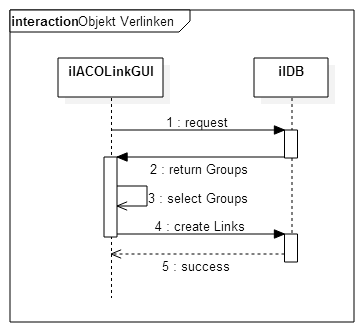
\includegraphics[width=.7\textwidth]{img/seq_linkGUI.png}
	\caption{Sequenzdiagramm Test verlinken}
\end{figure}
\begin{figure}[h!]
	\centering
	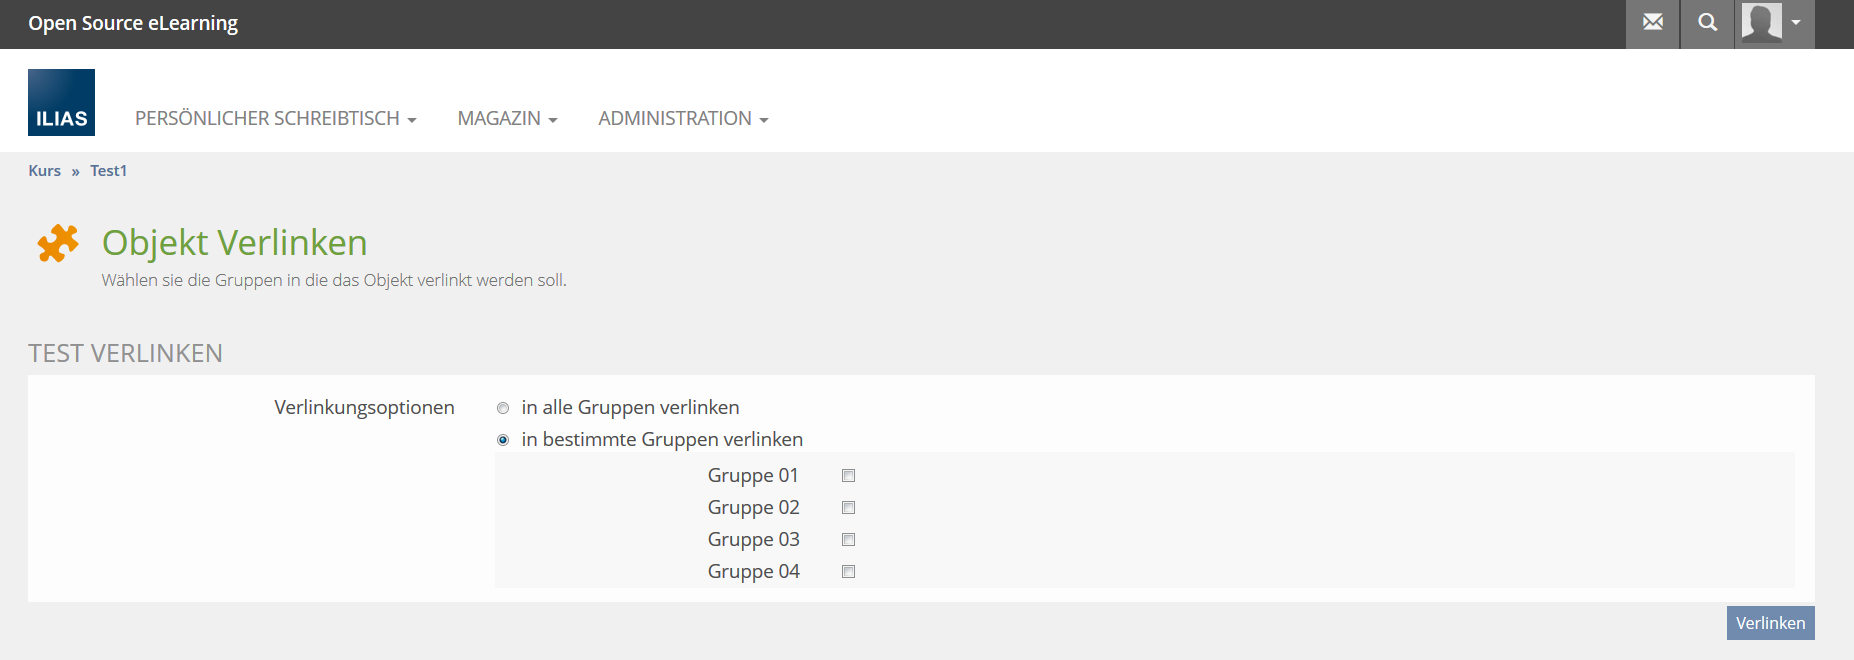
\includegraphics[width=1\textwidth]{img/linkTest.png}
	\caption{Ansicht Link Test}
\end{figure}

~\\Über einen Test gelangen wir über den Tab Verlinkung zu dem dargestellten Bild. 
Mit der Funktion lässt sich dieser Test in die Gruppen des Kurses in dem die Übung existiert verlinken/verknüpfen. 

\newpage

\subsection*{in alle Gruppen verlinken}
\begin{itemize}
	\item Sollte dieser Radio Button ausgewählt und auf verlinken geklickt werden, so wird diese Übung in alle im Kurs vorhandenen Gruppen verlinkt. 
\end{itemize}

\subsection*{in bestimmte Gruppen verlinken}
\begin{itemize}
	\item Sollte dieser Radio Button ausgewählt werden erscheint eine Auswahl aller im Kurs vorhandenen Gruppen mit einer Checkbox
	\item Man kann jetzt einzelne Gruppen via der Checkbox markieren
	\item Klickt man auf "Verlinken" werden diese Gruppen verlinkt
\end{itemize}

~\\(Achtung: Duplikate werden von diesem Tab ausgeschlossen bzw. es wird nicht doppelt verlinkt, sollte der Test schon in diese Gruppe verlinkt worden sein) 
\clearpage